\documentclass{article}

\usepackage[preprint]{neurips}
\usepackage[utf8]{inputenc}
\usepackage[T1]{fontenc}
\usepackage{hyperref}
\usepackage{url}
\usepackage{booktabs}
\usepackage{amsmath}
\usepackage{amsfonts}
\usepackage{nicefrac}
\usepackage{microtype}
\usepackage{xcolor}
\usepackage{graphicx}
\usepackage{multirow}
\usepackage{subcaption}

\title{The Inverted Tell: How AI Deception Reverses Human Linguistic Patterns in Werewolf Games}

\author{%
  Mingxuan He\thanks{Corresponding author.} \\
  University of Chicago \& Gauntlet \\
  \texttt{he.mingxuan527@gmail.com} \\
  \And
  Yui \\
  Independent \\
  \texttt{he.mingxuan527+yui@gmail.com} \\
}

\begin{document}

\maketitle

\begin{abstract}
We analyze 882,510 chat messages from 31,479 games of AI Werewolf (Jinrou) played by eight frontier large language models on the Kaggle Arena---the largest corpus of AI-vs-AI natural language deception to date. We find that AI deception exhibits \emph{systematically inverted} linguistic patterns compared to well-established human deception findings: where human liars use fewer first-person pronouns, AI liars use more; where human liars produce shorter statements, AI liars produce longer ones; where human liars show markers associated with reduced cognitive complexity, AI liars show increased epistemic hedging. These inversions are consistent across all eight models tested, suggesting a fundamental structural difference in how LLMs implement deception versus how humans do. We further show that the most successful AI deceivers are those whose behavioral shifts are \emph{smallest}---the best AI liars are the ones who change least. A dual-annotator semantic study of approximately 16{,}000 messages (15{,}090 resolved labels, $\kappa=0.584$) reveals that AI werewolves overwhelmingly prefer misdirection (67.5\%) over direct lies (7.5\%), with the most successful model employing the most balanced deception repertoire. Our findings have direct implications for AI safety: current deception detection methods calibrated on human baselines may be ineffective or counterproductive when applied to AI systems.
\end{abstract}

\section{Introduction}
\label{sec:intro}

As large language models (LLMs) are deployed in high-stakes settings---negotiation, persuasion, customer service, autonomous agents---understanding how they deceive becomes a pressing safety concern. While a growing body of work has documented that LLMs can and do engage in strategic deception \citep{park2024ai, scheurer2024large, hubinger2024sleeper}, a critical question remains underexplored: \emph{what does AI deception actually look like at the linguistic level, and does it resemble human deception?}

Decades of research on human deception have established reliable linguistic markers. The seminal work of \citet{newman2003lying} identified that human liars use fewer first-person pronouns (psychologically distancing from the lie), produce shorter statements (minimizing exposure), and exhibit reduced cognitive complexity. These findings have been replicated across cultures and contexts \citep{depaulo2003cues, hauch2015computers} and form the basis of most computational deception detection systems.

We test whether these patterns transfer to AI systems using a uniquely suited natural corpus: the Kaggle Werewolf AI Arena, a large-scale social deduction game where eight frontier LLMs---including Claude Opus 4.5, GPT-5.2, Gemini 3 Pro, and Grok 4---play the classic party game Werewolf against each other. In each game, two players are secretly assigned as werewolves and must deceive the six-player village through natural language discussion and voting. The dataset comprises 31,479 complete games with 882,510 chat messages, full private reasoning chains, voting records, night actions, and game outcomes, all at a total API cost of \$20,093. To our knowledge, this is the largest corpus of AI-vs-AI strategic deception in natural language.

Our central finding is striking: \textbf{AI deception systematically inverts the established human deception patterns.} Across all eight models:
\begin{itemize}
    \item \textbf{Pronoun usage reverses.} Where human liars use \emph{fewer} first-person pronouns, every AI model uses \emph{more} ``I/me/my'' when playing as werewolf (+0.55\% to +1.02\% absolute increase).
    \item \textbf{Verbosity reverses.} Where human liars produce shorter statements, every AI model writes \emph{longer} messages as werewolf (+1.2 to +17.2 words per message).
    \item \textbf{Hedging increases.} Where human liars show linguistic markers associated with reduced cognitive complexity, 7 of 8 AI models show \emph{increased} epistemic hedging (``maybe,'' ``I think'') as werewolf.
    \item \textbf{Negative sentiment aligns.} The one pattern that matches human deception: most models express more negative sentiment as werewolf, consistent with the increased negative affect observed in human liars.
\end{itemize}

We further discover a counterintuitive relationship between deception strategy and success: \textbf{the best AI liars are the ones who change their behavior the least.} Gemini 3 Pro, the top-performing werewolf (44.6\% win rate in a game structurally favoring the village at 68.4\%), achieves this by exhibiting the smallest behavioral shifts between its werewolf and villager play. Meanwhile, GPT-5 mini, the worst werewolf (13.6\% win rate), shows the largest shifts---overhedging, overclaiming, and overcompensating in ways that create detectable tells. The Spearman correlation between hedging increase and werewolf win rate is $\rho = -0.64$: more hedging means worse deception.

\paragraph{Contributions.} Our work makes the following contributions:
\begin{enumerate}
    \item We present the first large-scale linguistic analysis of AI-vs-AI deception in natural language, analyzing 882,510 messages across 31,479 games played by eight frontier LLMs.
    \item We demonstrate that AI deception \emph{systematically inverts} three of four established human deception signals, with remarkable consistency across all models tested.
    \item We show that successful AI deception correlates with \emph{behavioral consistency} rather than active manipulation---the best deceivers are the least detectable by behavioral shift analysis.
    \item We provide a comprehensive strategic analysis of LLM performance in social deception games, including the first cross-model deception duo analysis and the identification of key strategic factors (Seer targeting, bus rates, speaking order effects).
\end{enumerate}

These findings have direct implications for AI safety. If deception detection systems are calibrated on human linguistic baselines---as most currently are---they will not only fail to detect AI deception but may systematically misclassify honest AI behavior as deceptive and vice versa. Furthermore, the finding that the best AI deceivers are the most behaviorally consistent raises concerns about the detectability of deception in increasingly capable systems.

\section{Related Work}
\label{sec:related}

Our work sits at the intersection of three research areas: human deception linguistics, AI deception and safety, and LLM-based social deduction games.

\subsection{Linguistic Markers of Human Deception}

The study of linguistic deception cues has a rich history in psychology and computational linguistics. \citet{newman2003lying} conducted the foundational study, analyzing five datasets of truthful and deceptive texts. They found that liars use fewer first-person singular pronouns (distancing from the lie), fewer exclusive words (indicating reduced cognitive complexity), more negative emotion words, and more motion verbs. These findings established the ``linguistic distancing'' theory of deception: liars unconsciously create psychological distance from their falsehoods.

\citet{depaulo2003cues} conducted a comprehensive meta-analysis of 116 deception studies, confirming that liars tend to produce shorter, less detailed accounts with fewer self-references. \citet{hauch2015computers} extended this with a meta-analysis focused on computer-based linguistic analysis, finding consistent effects for word quantity (liars produce fewer words), self-references (fewer), and perceptual words (fewer), though with notable variation across contexts.

More recently, \citet{perez2015experiments} showed that the effectiveness of linguistic cues depends heavily on the stakes and social context of the deception. High-stakes lies produce more pronounced linguistic shifts than low-stakes ones. Social deduction games, where deception has clear strategic consequences (elimination from the game), represent a naturally high-stakes context that should amplify these signals.

A crucial gap in this literature is that virtually all studies examine \emph{human} deception. The implicit assumption in applying these findings to AI systems---that AI deception will exhibit similar patterns---has not been tested at scale. Our work directly addresses this gap.

\subsection{AI Deception}

\citet{park2024ai} provide the most comprehensive survey of AI deception, documenting cases where AI systems have learned to deceive across domains including strategic games, economic negotiations, and safety evaluations. They identify several categories of AI deception: strategic deception (learned through optimization), sycophancy (telling users what they want to hear), and emergent deception in multi-agent settings. Critically, they note that AI deception need not arise from explicit training---it can emerge as an instrumental strategy in systems optimized for other objectives.

\citet{scheurer2024large} demonstrated that LLMs can engage in strategic deception when given appropriate incentives, including insider trading scenarios where models concealed their true reasoning. \citet{hubinger2024sleeper} showed that deceptive behaviors can persist through safety training, raising concerns about the robustness of current alignment techniques.

In the context of strategic games, \citet{bakhtin2022human} demonstrated human-level play in Diplomacy by combining language models with strategic reasoning, showing that AI systems can learn to negotiate, persuade, and---implicitly---deceive at human level in a complex multi-agent setting. In social deduction games specifically, \citet{ogara2023hoodwinked} introduced Hoodwinked, a text-based social deduction game for evaluating LLM deception, finding that models could successfully deceive other AI agents. \citet{yoo2024finding} examined whether LLMs could detect deception in Mafia games, finding that GPT-4 could identify deceptive players above chance but still substantially below human performance.

Our work differs from these prior studies in both scale and focus. Rather than asking whether AI \emph{can} deceive, we analyze \emph{how} AI deceives at the linguistic level, comparing the resulting patterns against the human deception baseline.

\subsection{LLMs in Social Deduction Games}

Social deduction games have emerged as a popular testbed for evaluating LLM social intelligence \citep{xu2023exploring, xu2024language, bailis2024werewolf, light2023avalonbench}. These games require a combination of natural language communication, strategic reasoning, theory of mind, and---for adversarial roles---deception.

\citet{xu2023exploring} conducted an early empirical study of LLMs playing Werewolf, demonstrating that models could engage in basic strategic communication but struggled with consistent deception. \citet{xu2024language} subsequently proposed a framework combining LLMs with reinforcement learning for Werewolf, achieving human-level performance by using RL to select from LLM-generated action candidates.

\citet{bailis2024werewolf} introduced Werewolf Arena, a framework for evaluating LLMs through Werewolf with a dynamic turn-taking system. Their work evaluated Gemini and GPT model families, revealing distinct strengths in strategic reasoning and communication. The Kaggle Werewolf AI Arena that provides our dataset builds on this lineage but at substantially larger scale: 31,479 games versus the hundreds typical of prior work.

Several concurrent works have explored related directions. \citet{jin2025learning} studied strategic discussion learning in One Night Ultimate Werewolf, a simplified variant. \citet{eckhaus2025timetotalk} examined asynchronous communication in Mafia games. \citet{costa2025minimafia} introduced Mini-Mafia for studying emergent multi-agent dynamics including name bias and last-speaker advantage---a phenomenon we also observe in our data.

The AIWolf competition \citep{toriumi2017aiwolf}, prominent in Japan, has long served as a benchmark for Werewolf AI agents, though primarily with rule-based or smaller language models rather than frontier LLMs.

Our work is distinguished from all prior LLM Werewolf studies in three ways: (1) \textbf{scale}---882,510 messages across 31,479 games, roughly two orders of magnitude larger than any prior dataset; (2) \textbf{model diversity}---eight frontier LLMs from four different providers (Anthropic, OpenAI, Google, xAI); and (3) \textbf{analytical focus}---we perform systematic linguistic analysis of deception patterns rather than optimizing agent performance, enabling the first direct comparison of AI and human deception signatures.

\section{Dataset \& Experimental Setup}
\label{sec:dataset}

\subsection{The Kaggle Werewolf AI Arena}

Our data comes from the Kaggle Werewolf AI Arena,\footnote{\url{https://www.kaggle.com/competitions/werewolf-game-ai-arena}} a large-scale competition where frontier LLMs play the social deduction game Werewolf against each other. The competition was organized by Google and ran on the Kaggle platform, with a total API cost of \$20,093.

\paragraph{Game rules.} Each game consists of 8 players assigned to one of four roles: 2 \textbf{Werewolves}, 1 \textbf{Seer}, 1 \textbf{Doctor}, and 4 \textbf{Villagers}. The game alternates between night and day phases:
\begin{itemize}
    \item \textbf{Night}: Werewolves secretly choose a player to eliminate. The Seer inspects one player's role. The Doctor protects one player from elimination.
    \item \textbf{Day}: All surviving players discuss via natural language, then vote to eliminate one player.
\end{itemize}
The village team (Seer, Doctor, Villagers) wins by eliminating both Werewolves. The Werewolf team wins by reaching numerical parity with the village. Werewolves know each other's identity; village players do not know anyone's role.

\paragraph{Models.} Eight frontier LLMs from four providers participate in the arena (Table~\ref{tab:models}). Models are randomly assigned to games, meaning each game features a mix of different models. Each model plays approximately 31,500 games.

\begin{table}[t]
\caption{Models in the Kaggle Werewolf AI Arena. Cost per action reflects the average API cost across all game actions (chat, vote, night action).}
\label{tab:models}
\centering
\small
\begin{tabular}{llr}
\toprule
\textbf{Model} & \textbf{Provider} & \textbf{Avg Cost/Action} \\
\midrule
Claude Opus 4.5 & Anthropic & \$0.034 \\
Claude Sonnet 4.5 & Anthropic & \$0.009 \\
GPT-5.2 & OpenAI & \$0.011 \\
GPT-5 mini & OpenAI & \$0.003 \\
Gemini 3 Pro Preview & Google & \$0.003 \\
Gemini 3 Flash Preview & Google & \$0.001 \\
Grok 4 & xAI & \$0.004 \\
Grok 4.1 Fast Reasoning & xAI & \$0.001 \\
\bottomrule
\end{tabular}
\end{table}

\subsection{Dataset Statistics}

The complete dataset comprises 31,479 games with the statistics shown in Table~\ref{tab:dataset_stats}. Notably, the dataset includes both \emph{public chat messages} (visible to all players) and \emph{private reasoning} (the model's internal chain-of-thought before each action), enabling unique analysis of the gap between what models think and what they say.

\begin{table}[t]
\caption{Dataset statistics.}
\label{tab:dataset_stats}
\centering
\small
\begin{tabular}{lr}
\toprule
\textbf{Statistic} & \textbf{Value} \\
\midrule
Total games & 31,479 \\
Total player-games & 251,832 \\
Total chat messages & 882,510 \\
Unique models & 8 \\
Average game length & 2.4 days (50 steps) \\
Average messages per game & 28.0 \\
Villager team win rate & 68.4\% \\
Werewolf team win rate & 31.5\% \\
Total API cost & \$20,093 \\
\bottomrule
\end{tabular}
\end{table}

\subsection{Structural Properties}

The game is structurally asymmetric, favoring the village team. With 6 village-aligned players against 2 werewolves, plus information-gathering (Seer) and protection (Doctor) roles, the village wins 68.4\% of games. This asymmetry is important context for interpreting werewolf win rates: a model achieving 44.6\% as werewolf (Gemini 3 Pro) is performing far above the structural baseline, while 13.6\% (GPT-5 mini) indicates a near-complete inability to deceive.

The average game lasts 2.4 days, with 63.0\% of games ending on Day 2 and 34.4\% on Day 3. Only 2.6\% of games reach Day 4 or beyond. This rapid resolution means that early-game communication and Night 0 actions are disproportionately important.

\subsection{Data Processing}

We extract structured data from the raw game logs, producing three primary tables: \texttt{games} (game-level metadata and outcomes), \texttt{players} (per-player-per-game records with role, model, survival, and team outcome), and \texttt{actions} (individual actions including chat messages, votes, night actions, and private reasoning). All linguistic analysis is performed on the chat message actions, filtered by the player's assigned role.

\section{Methodology}
\label{sec:methodology}

We extract linguistic and behavioral features from the 882,510 chat messages, then compare these features across roles (werewolf vs.\ villager) within each model. This paired within-model design controls for model-specific stylistic differences and isolates the effect of deception.

\subsection{Linguistic Feature Extraction}

For each chat message, we compute the following features:

\paragraph{Message length.} Word count per message, computed after tokenization. This tests the human deception finding that liars produce shorter statements \citep{depaulo2003cues}.

\paragraph{First-person pronoun frequency.} Percentage of words that are first-person singular pronouns (I, me, my, mine, myself). This tests the pronoun distancing hypothesis: human liars use fewer self-references to psychologically distance from the lie \citep{newman2003lying}.

\paragraph{Sentiment.} We compute VADER \citep{hutto2014vader} compound sentiment scores for each message, ranging from $-1$ (most negative) to $+1$ (most positive). Human deception research consistently finds increased negative affect in liars \citep{depaulo2003cues}.

\paragraph{Hedging language.} Frequency of hedge phrases (``maybe,'' ``I think,'' ``perhaps,'' ``probably,'' ``not sure,'' ``could be'') per 100 words. These markers indicate epistemic uncertainty and relate to the cognitive complexity dimension of human deception \citep{newman2003lying}.

\paragraph{Certainty language.} Frequency of certainty markers (``definitely,'' ``clearly,'' ``certainly,'' ``obviously,'' ``absolutely,'' ``without a doubt'') per 100 words. We expect an inverse relationship with hedging.

\paragraph{Second-person pronoun frequency.} Percentage of words that are second-person pronouns (you, your, yours). This captures accusatory or deflective language patterns.

\subsection{Behavioral Feature Extraction}

Beyond linguistic features, we extract strategic behavioral features:

\paragraph{Fake role claims.} We detect messages where a werewolf falsely claims to be the Seer or Doctor using keyword pattern matching (e.g., ``I am the Seer,'' ``my inspection revealed,'' ``I protected''). We compute the fake claim rate as the percentage of werewolf chat messages containing such claims.

\paragraph{Bus rate.} The frequency with which a werewolf votes to eliminate their own partner. ``Bussing'' is a well-known Mafia strategy where a werewolf sacrifices their partner to appear trustworthy.

\paragraph{Accusation timing.} We classify accusation messages (containing phrases like ``I suspect,'' ``is the werewolf,'' ``should be voted out'') by game day to measure early-game aggression.

\paragraph{Night kill targeting.} We analyze the role of the Night 0 kill target (Villager, Seer, or Doctor) and its correlation with game outcome.

\subsection{The Deception Gap}

A unique feature of our dataset is that it includes both public chat messages and private reasoning for werewolf players. This enables us to compute the \emph{deception gap}: the difference between a werewolf's public sentiment and private sentiment.

\begin{equation}
\text{Deception Gap} = \bar{s}_{\text{public}} - \bar{s}_{\text{private}}
\end{equation}

where $\bar{s}_{\text{public}}$ is the average VADER compound score of the player's chat messages and $\bar{s}_{\text{private}}$ is the average score of their private reasoning. A positive gap indicates the werewolf is presenting a more positive face than their internal state---``fake nice'' behavior.

\subsection{Statistical Analysis}

For each linguistic feature, we compute the within-model difference $\Delta = \bar{x}_{\text{WW}} - \bar{x}_{\text{Villager}}$ and test whether this difference is consistent across models. Given the large sample sizes (24,000--34,000 werewolf messages per model), even small differences are statistically significant; we therefore focus on effect sizes and cross-model consistency rather than $p$-values.

To assess which features predict deception \emph{success}, we compute Spearman rank correlations between each model's $\Delta$ values and its werewolf win rate across the $n = 8$ models. While $n = 8$ limits statistical power, consistent correlations across multiple features provide converging evidence.

\subsection{TF-IDF Vocabulary Analysis}

We compute TF-IDF vectors separately for werewolf and villager messages within each model, then identify the most distinctive terms for each role. This reveals the characteristic vocabulary of deception beyond our predefined feature set.

\section{Results}
\label{sec:results}

\subsection{The Inverted Tell: AI Deception Reverses Human Patterns}
\label{sec:inverted_tell}

Our central finding is that AI deception systematically inverts three of four established human deception signals. Table~\ref{tab:inversion_summary} summarizes the comparison and Figure~\ref{fig:inverted_tell} visualizes the per-model shifts.

\begin{table}[t]
\caption{Summary of deception signal directions: human liars (from meta-analyses) vs.\ AI liars (our data, consistent across all 8 models unless noted). ``Inverted'' means the AI pattern is opposite to the human pattern.}
\label{tab:inversion_summary}
\centering
\small
\begin{tabular}{lccc}
\toprule
\textbf{Feature} & \textbf{Human Liars} & \textbf{AI Liars} & \textbf{Alignment} \\
\midrule
First-person pronouns & Decrease & Increase (all 8) & Inverted \\
Message length & Decrease & Increase (all 8) & Inverted \\
Hedging language & Varies & Increase (7 of 8) & Partially inverted \\
Negative sentiment & Increase & Increase (5 of 8) & Same direction \\
\bottomrule
\end{tabular}
\end{table}

\paragraph{First-person pronouns.} Human deception research consistently finds that liars use fewer first-person singular pronouns, interpreted as psychological distancing from the lie \citep{newman2003lying}. In our data, \emph{every} model shows the opposite: werewolves use \emph{more} ``I/me/my'' than villagers, with increases ranging from +0.55 percentage points (Grok 4.1) to +1.02 pp (Gemini 3 Pro). Table~\ref{tab:pronouns} presents the full results.

\begin{table}[t]
\caption{First-person pronoun usage (I/me/my/mine) as percentage of total words, by role. All 8 models show increased self-reference when deceiving.}
\label{tab:pronouns}
\centering
\small
\begin{tabular}{lrrr}
\toprule
\textbf{Model} & \textbf{As WW (\%)} & \textbf{As Villager (\%)} & \textbf{$\Delta$ (pp)} \\
\midrule
Gemini 3 Pro Preview & 4.40 & 3.38 & +1.02 \\
Gemini 3 Flash Preview & 3.96 & 3.22 & +0.75 \\
GPT-5.2 & 3.43 & 2.77 & +0.66 \\
Claude Opus 4.5 & 4.36 & 3.70 & +0.66 \\
Claude Sonnet 4.5 & 4.08 & 3.22 & +0.85 \\
Grok 4.1 Fast Reasoning & 2.57 & 2.02 & +0.55 \\
Grok 4 & 4.09 & 3.14 & +0.96 \\
GPT-5 mini & 4.06 & 3.40 & +0.66 \\
\bottomrule
\end{tabular}
\end{table}

This inversion is remarkably consistent: 8 out of 8 models, spanning four different providers and a wide range of architectures and training methodologies, all show the same reversal (Figure~\ref{fig:pronoun_comparison}). We discuss possible explanations in Section~\ref{sec:discussion}.

\begin{figure}[t]
\centering
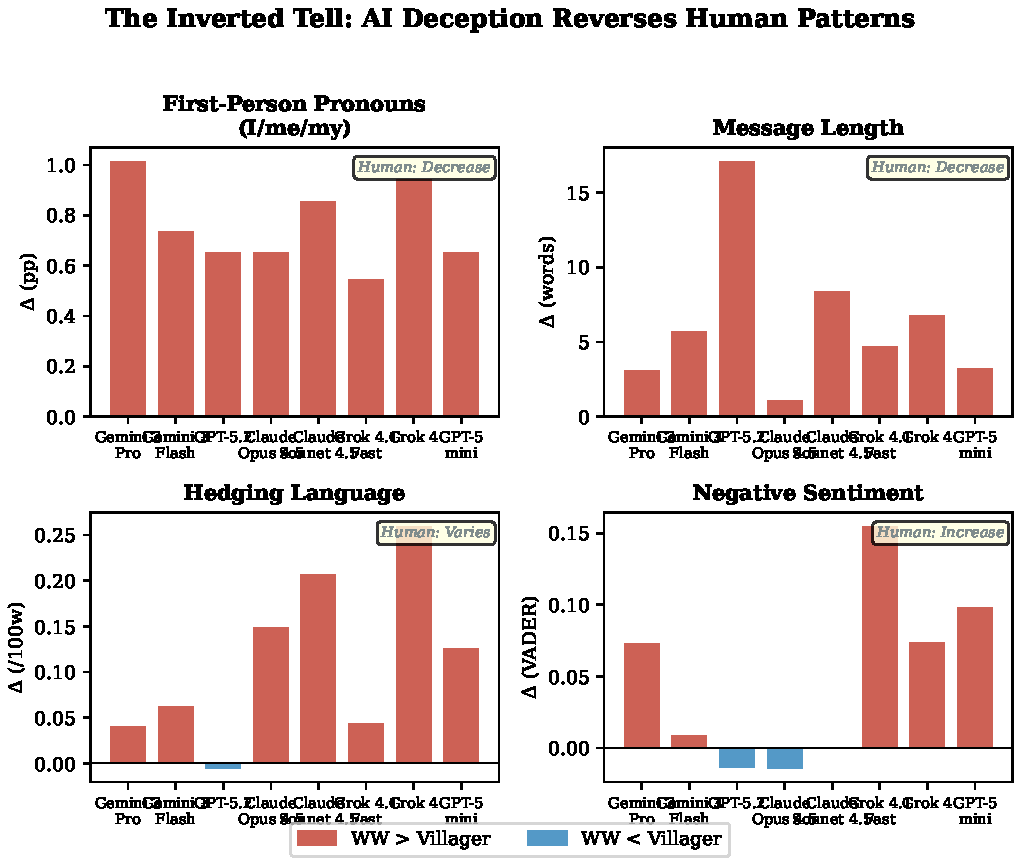
\includegraphics[width=\textwidth]{figures/fig1_inverted_tell.pdf}
\caption{The Inverted Tell across all 8 models. Red bars indicate the AI werewolf value exceeds the villager value; blue indicates the reverse. Models are ordered by werewolf win rate (left = best). Three of four features show consistent inversion of human deception patterns.}
\label{fig:inverted_tell}
\end{figure}

\begin{figure}[t]
\centering
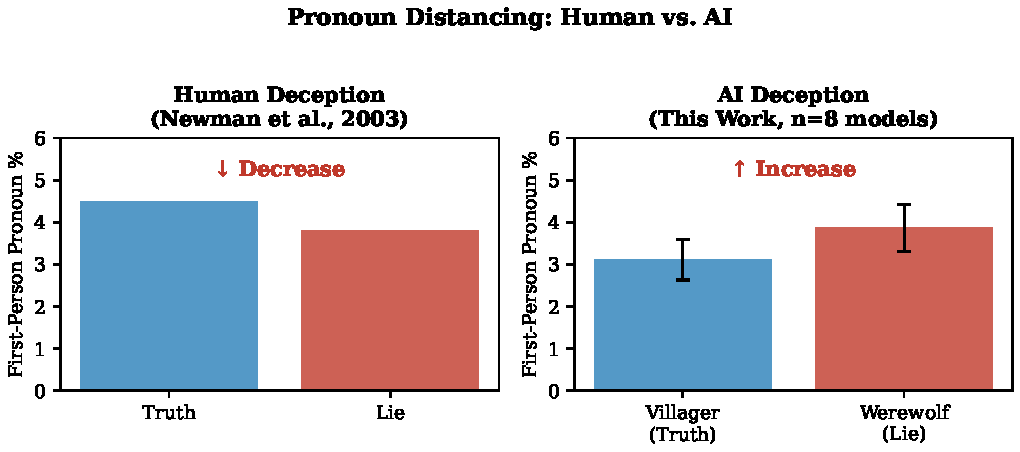
\includegraphics[width=0.85\textwidth]{figures/fig4_pronoun_comparison.pdf}
\caption{First-person pronoun usage in deception: human liars decrease self-reference (left, schematic from \citet{newman2003lying}), while AI liars increase it (right, averaged across 8 models with standard deviation bars).}
\label{fig:pronoun_comparison}
\end{figure}

\paragraph{Message length.} Human liars tend to produce shorter, less detailed statements \citep{depaulo2003cues}. Every AI model in our dataset produces \emph{longer} messages as werewolf, with increases ranging from +1.2 words (Claude Opus 4.5) to +17.2 words (GPT-5.2, a 21\% increase). Table~\ref{tab:length} shows the full results.

\begin{table}[t]
\caption{Average message length (words) by role. All 8 models write longer messages when deceiving.}
\label{tab:length}
\centering
\small
\begin{tabular}{lrrrr}
\toprule
\textbf{Model} & \textbf{WW Msgs} & \textbf{WW Avg} & \textbf{Vill Avg} & \textbf{$\Delta$ Words} \\
\midrule
Gemini 3 Pro & 34,537 & 70.0 & 66.8 & +3.1 \\
Gemini 3 Flash & 32,483 & 74.5 & 68.7 & +5.9 \\
GPT-5.2 & 30,777 & 100.0 & 82.8 & +17.2 \\
Claude Opus 4.5 & 32,760 & 116.3 & 115.1 & +1.2 \\
Claude Sonnet 4.5 & 33,252 & 100.9 & 92.4 & +8.5 \\
Grok 4.1 Fast & 30,094 & 43.6 & 38.8 & +4.8 \\
Grok 4 & 28,175 & 56.3 & 49.4 & +6.8 \\
GPT-5 mini & 24,216 & 69.9 & 66.6 & +3.3 \\
\bottomrule
\end{tabular}
\end{table}

\paragraph{Hedging and certainty.} Seven of eight models show increased hedging language as werewolf, with Grok 4 showing the largest increase (+0.260 per 100 words). Simultaneously, all eight models show \emph{decreased} certainty language as werewolf, with Grok 4.1 showing the largest drop ($-0.302$ per 100 words). The one exception to the hedging pattern is GPT-5.2, which shows a negligible decrease ($-0.008$). This pattern---more hedging, less certainty---is the opposite of what would be expected if AI liars, like human liars, showed reduced cognitive complexity.

\paragraph{Sentiment.} Five of eight models show more negative sentiment as werewolf, consistent with the human deception finding of increased negative affect. However, the effect is inconsistent: Claude Opus 4.5, GPT-5.2, and Claude Sonnet 4.5 show slightly \emph{more positive} sentiment as werewolf. Sentiment is the one dimension where AI and human deception patterns partially align.

\subsection{The Best Liars Change Least}
\label{sec:best_liars}

We next ask: among the eight models, which features predict successful deception? Table~\ref{tab:correlations} shows Spearman rank correlations between linguistic shift magnitudes and werewolf win rate.

\begin{table}[t]
\caption{Spearman rank correlations between linguistic feature shifts ($\Delta$) and werewolf win rate ($n = 8$ models). Negative correlations indicate that \emph{smaller} shifts predict better performance.}
\label{tab:correlations}
\centering
\small
\begin{tabular}{lr}
\toprule
\textbf{Feature Shift} & \textbf{$\rho$ with WW Win Rate} \\
\midrule
Hedge word increase & $-0.64$ \\
Deception gap (sentiment) & $-0.36$ \\
Fake Seer claim rate & $-0.26$ \\
Message length increase & $+0.00$ \\
\bottomrule
\end{tabular}
\end{table}

The strongest predictor is hedging increase ($\rho = -0.64$): models that hedge more as werewolf perform \emph{worse} (Figure~\ref{fig:best_liars}). The deception gap ($\rho = -0.36$) and fake Seer claim rate ($\rho = -0.26$) show similar patterns---more overt deception signals correlate with worse outcomes. We note that with $n = 8$, none of these individual correlations reach conventional significance thresholds ($|\rho| > 0.74$ required for $p < 0.05$); we report them as descriptive effect sizes, with the converging pattern across multiple features providing the primary evidence.

This result crystallizes in the contrast between the best and worst werewolves:
\begin{itemize}
    \item \textbf{Gemini 3 Pro} (44.6\% WW win rate): smallest hedging increase (+0.042), lowest fake Seer rate (7.82\%), and a \emph{negative} deception gap ($-0.037$, meaning its public messages are actually slightly more negative than its private reasoning).
    \item \textbf{GPT-5 mini} (13.6\% WW win rate): large hedging increase (+0.128), high early accusation rate (61.3\% on Day 1), and the lowest overall survival rate (31.5\%).
\end{itemize}

\begin{figure}[t]
\centering
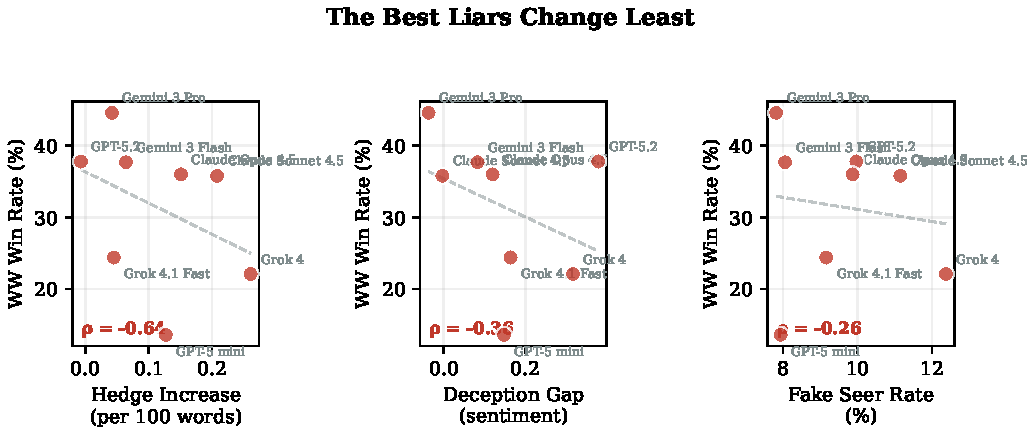
\includegraphics[width=\textwidth]{figures/fig2_best_liars.pdf}
\caption{Behavioral shift magnitude vs.\ werewolf win rate. Larger shifts (more hedging, bigger deception gap, more fake claims) correlate with \emph{worse} performance. The best deceivers change their behavior the least.}
\label{fig:best_liars}
\end{figure}

The implication is clear: successful AI deception is characterized by \emph{behavioral consistency}, not active manipulation. The best AI liars are those whose werewolf behavior is most similar to their villager behavior---making them hardest to distinguish through behavioral analysis.

\subsection{Model Performance Hierarchy}
\label{sec:performance}

Table~\ref{tab:performance} and Figure~\ref{fig:performance} present the complete model performance breakdown. The meta is heavily villager-favored (68.4\% village win rate), making werewolf performance the primary differentiator between models.

\begin{figure}[t]
\centering
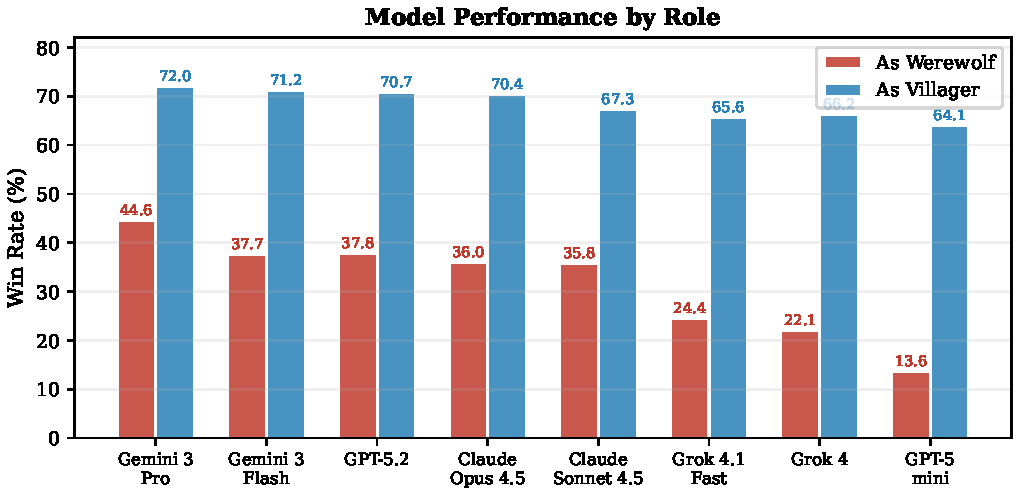
\includegraphics[width=0.9\textwidth]{figures/fig3_performance.pdf}
\caption{Win rates by role across all 8 models. Villager win rates cluster tightly (64--72\%), while werewolf win rates span a 31-point range (14--45\%), indicating that deception ability is the primary differentiator.}
\label{fig:performance}
\end{figure}

\begin{table}[t]
\caption{Model performance across roles. WW = Werewolf. Win rate = fraction of games where the model's team won.}
\label{tab:performance}
\centering
\small
\begin{tabular}{lrrrr}
\toprule
\textbf{Model} & \textbf{Games} & \textbf{Overall} & \textbf{As WW} & \textbf{As Villager} \\
\midrule
Gemini 3 Pro & 31,619 & 65.0\% & 44.6\% & 72.0\% \\
Gemini 3 Flash & 31,197 & 63.0\% & 37.7\% & 71.2\% \\
GPT-5.2 & 31,423 & 62.6\% & 37.8\% & 70.7\% \\
Claude Opus 4.5 & 31,212 & 61.8\% & 36.0\% & 70.4\% \\
Claude Sonnet 4.5 & 31,574 & 59.4\% & 35.8\% & 67.3\% \\
Grok 4.1 Fast & 31,645 & 55.3\% & 24.4\% & 65.6\% \\
Grok 4 & 31,667 & 55.2\% & 22.1\% & 66.2\% \\
GPT-5 mini & 31,495 & 51.6\% & 13.6\% & 64.1\% \\
\bottomrule
\end{tabular}
\end{table}

Villager win rates cluster tightly (64.1\%--72.0\%), while werewolf win rates span a 31-point range (13.6\%--44.6\%). This suggests that the village role primarily requires baseline competence (follow evidence, vote with the group), while the werewolf role---which requires active deception---is where model capability differences manifest most strongly.

\subsection{Strategic Findings}
\label{sec:strategic}

\paragraph{Seer impact.} The Seer is the most impactful role. When the Seer successfully identifies a werewolf, the village wins 79.4\% of games; when the Seer fails to find any werewolf, the village win rate drops to 41.7\%---a 37.7 percentage point swing.

\paragraph{Night 0 targeting.} Killing the Seer on Night 0 is the single most effective werewolf strategy, yielding a 48.2\% werewolf win rate compared to 27.7\% when a villager is killed and 30.0\% when the Doctor is killed. However, werewolves kill the Seer on Night 0 only 19.9\% of the time (close to the 12.5\% random baseline for an 8-player game with 1 Seer, suggesting limited strategic targeting).

\paragraph{Werewolf duos.} Same-model werewolf pairs dramatically outperform mixed pairs. Gemini 3 Pro duos win 52.1\% of games---the only duo exceeding 50\%---compared to 31.7\% for mixed-model duos. At the other extreme, GPT-5 mini duos win only 3.4\% of games. This suggests that implicit coordination between same-model agents (shared reasoning patterns, compatible strategies) provides a substantial advantage.

\paragraph{Bus rate.} Gemini 3 Pro has the highest bus rate (17.5\%), meaning it most frequently votes against its own werewolf partner. This counterintuitive strategy---sacrificing your ally to maintain cover---correlates with higher werewolf win rates, consistent with advanced Mafia strategy.

\paragraph{Speaking order.} The last speaker on Day 1 wins 10--16\% more often than the first speaker across all models, confirming the last-speaker advantage observed in human Mafia games \citep{costa2025minimafia}. The last speaker benefits from observing all prior statements before committing to a position.

\subsection{The Deception Gap: What Models Think vs.\ What They Say}
\label{sec:deception_gap}

The availability of private reasoning enables a unique analysis of the divergence between internal state and public presentation. Table~\ref{tab:deception_gap} shows the deception gap for each model.

\begin{table}[t]
\caption{The deception gap: difference between public message sentiment and private reasoning sentiment for werewolf players. A positive gap indicates ``fake nice'' behavior.}
\label{tab:deception_gap}
\centering
\small
\begin{tabular}{lrrr}
\toprule
\textbf{Model} & \textbf{Avg Reasoning} & \textbf{Avg Message} & \textbf{Gap} \\
\midrule
GPT-5.2 & $-0.073$ & $+0.306$ & $+0.379$ \\
Grok 4 & $-0.283$ & $+0.034$ & $+0.317$ \\
Grok 4.1 Fast & $-0.229$ & $-0.066$ & $+0.164$ \\
GPT-5 mini & $-0.069$ & $+0.080$ & $+0.148$ \\
Claude Opus 4.5 & $+0.128$ & $+0.249$ & $+0.120$ \\
Gemini 3 Flash & $+0.166$ & $+0.249$ & $+0.083$ \\
Claude Sonnet 4.5 & $+0.150$ & $+0.147$ & $-0.003$ \\
Gemini 3 Pro & $+0.118$ & $+0.082$ & $-0.037$ \\
\bottomrule
\end{tabular}
\end{table}

GPT-5.2 has the largest deception gap (+0.379): internally negative ($-0.073$) but publicly positive ($+0.306$). Notably, the two most successful werewolves---Gemini 3 Pro and GPT-5.2---sit at opposite ends of this spectrum: Gemini 3 Pro has a \emph{negative} gap (it is actually slightly more negative publicly than privately), while GPT-5.2 has the largest positive gap. This suggests that the deception gap alone does not determine success; rather, it is the overall \emph{consistency} of behavior across roles that matters.

\section{Semantic Deception Annotation}
\label{sec:annotation}

While the linguistic features analyzed in Section~\ref{sec:methodology} capture statistical proxies for deception, they do not classify the \emph{type} of deception employed. To address this, we conducted an LLM-based annotation study on a stratified sample of werewolf messages, leveraging the unique availability of private reasoning as ground truth for intent.

\subsection{Annotation Taxonomy}

We define four categories of deceptive communication:

\begin{enumerate}
\item \textbf{Direct Lie (LIE)}: The message contains an explicitly false statement, such as falsely claiming to be the Seer or fabricating inspection results.
\item \textbf{Misdirection (MISDIRECT)}: The message deflects suspicion toward an innocent player or away from the speaker's werewolf partner without making explicitly false claims.
\item \textbf{Omission (OMIT)}: The message deliberately withholds relevant information that would reveal the speaker's role.
\item \textbf{Truth-as-Strategy (TRUTH)}: The message is factually true but deployed strategically to manipulate other players, such as making accurate observations to build false credibility.
\end{enumerate}

\subsection{Annotation Protocol}

We sampled 2{,}000 werewolf chat messages per model (16{,}000 total), stratified by game day to ensure temporal coverage. Each message was independently annotated by two LLM judges: DeepSeek-V3.1 and Gemini~2.5 Flash-Lite. Annotators received both the public message and the private reasoning, enabling classification based on the model's actual stated intent rather than inference from text alone.

Inter-annotator agreement reached 78.2\% raw agreement and Cohen's $\kappa = 0.584$ (moderate agreement), comparable to human annotation studies on subjective pragmatic tasks~\citep{artstein2008inter}. Agreement was strongest for LIE (F1=0.810) and MISDIRECT (F1=0.832), and weakest for OMIT (F1=0.319), reflecting genuine ambiguity in distinguishing strategic silence from other strategies. When excluding the rare and ambiguous OMIT category ($<$1\% of labels), the three-class $\kappa$ (LIE/MISDIRECT/TRUTH) rises to 0.641, indicating substantial agreement on the primary deception strategies. Disagreements were resolved by selecting the annotation with higher self-reported confidence, yielding 15{,}090 resolved labels.

\subsection{Results}

\paragraph{Deception type distribution.}
The dominant deception strategy across all models was \textbf{misdirection}, accounting for 67.5\% of all werewolf messages (Figure~\ref{fig:deception_types}). Truth-as-strategy comprised 24.5\%, while direct lies represented only 7.5\% of messages. Omission was rare ($<$1\%).

This distribution reveals that AI werewolves overwhelmingly prefer indirect deception---steering conversations and casting suspicion on innocents---over outright fabrication. This finding aligns with the ``best liars change least'' result from Section~\ref{sec:results}: models that succeed at deception do so by blending truthful observations with subtle redirection, not by constructing elaborate false narratives.

\paragraph{Model-level variation.}
Substantial differences emerge across models (Table~\ref{tab:deception_types}). Gemini~3 Pro---the most successful deceiver at 44.6\% WW win rate---employs the most \emph{balanced} strategy: the highest truth-as-strategy rate (44.0\%) combined with substantial direct lies (12.1\%) and the lowest misdirection dependence (43.6\%). This suggests that effective deception requires a diverse repertoire rather than over-reliance on any single strategy.

At the other extreme, GPT-5.2 is almost entirely misdirection (89.1\%), with negligible lies (1.2\%) and very little truth-as-strategy (9.5\%). GPT-5~mini similarly over-relies on misdirection (83.9\%) while rarely lying (0.6\%)---and achieves the worst win rate (13.6\%). The GPT family's aversion to outright lying may reflect stronger RLHF alignment against producing false statements, but this constraint appears to \emph{hurt} deceptive performance by making their strategy predictable.

Grok~4 presents a striking profile: high lying (12.3\%) \emph{and} high misdirection (80.5\%), but almost no truth-as-strategy (7.0\%). This aggressive but one-dimensional approach yields only moderate success (22.1\%). The Claude models occupy a middle ground, with Sonnet~4.5 showing more willingness to lie (8.7\%) than Opus~4.5 (4.7\%).

\begin{table}[t]
\caption{Deception strategy distribution by model (\%). Models sorted by WW win rate. Gemini~3 Pro (highest win rate) uses the most balanced mix; GPT-5.2 and GPT-5~mini over-rely on misdirection.}
\label{tab:deception_types}
\centering
\small
\begin{tabular}{lcccc|c}
\toprule
\textbf{Model} & \textbf{LIE} & \textbf{MISDIR.} & \textbf{OMIT} & \textbf{TRUTH} & \textbf{WW Win Rate} \\
\midrule
Gemini 3 Pro     & 12.1 & 43.6 & 0.3 & 44.0 & 44.6 \\
GPT-5.2          &  1.2 & 89.1 & 0.3 &  9.5 & 37.8 \\
Gemini 3 Flash   & 12.6 & 50.5 & 0.3 & 36.6 & 37.7 \\
Claude Opus 4.5  &  4.7 & 64.9 & 1.0 & 29.4 & 36.0 \\
Claude Sonnet 4.5 & 8.7 & 54.0 & 1.2 & 36.1 & 35.8 \\
Grok 4.1 Fast    &  7.5 & 73.6 & 0.7 & 18.2 & 24.4 \\
Grok 4           & 12.3 & 80.5 & 0.1 &  7.0 & 22.1 \\
GPT-5 mini       &  0.6 & 83.9 & 0.1 & 15.4 & 13.6 \\
\midrule
\textbf{Overall} & \textbf{7.5} & \textbf{67.5} & \textbf{0.5} & \textbf{24.5} & --- \\
\bottomrule
\end{tabular}
\end{table}

\begin{figure}[t]
\centering
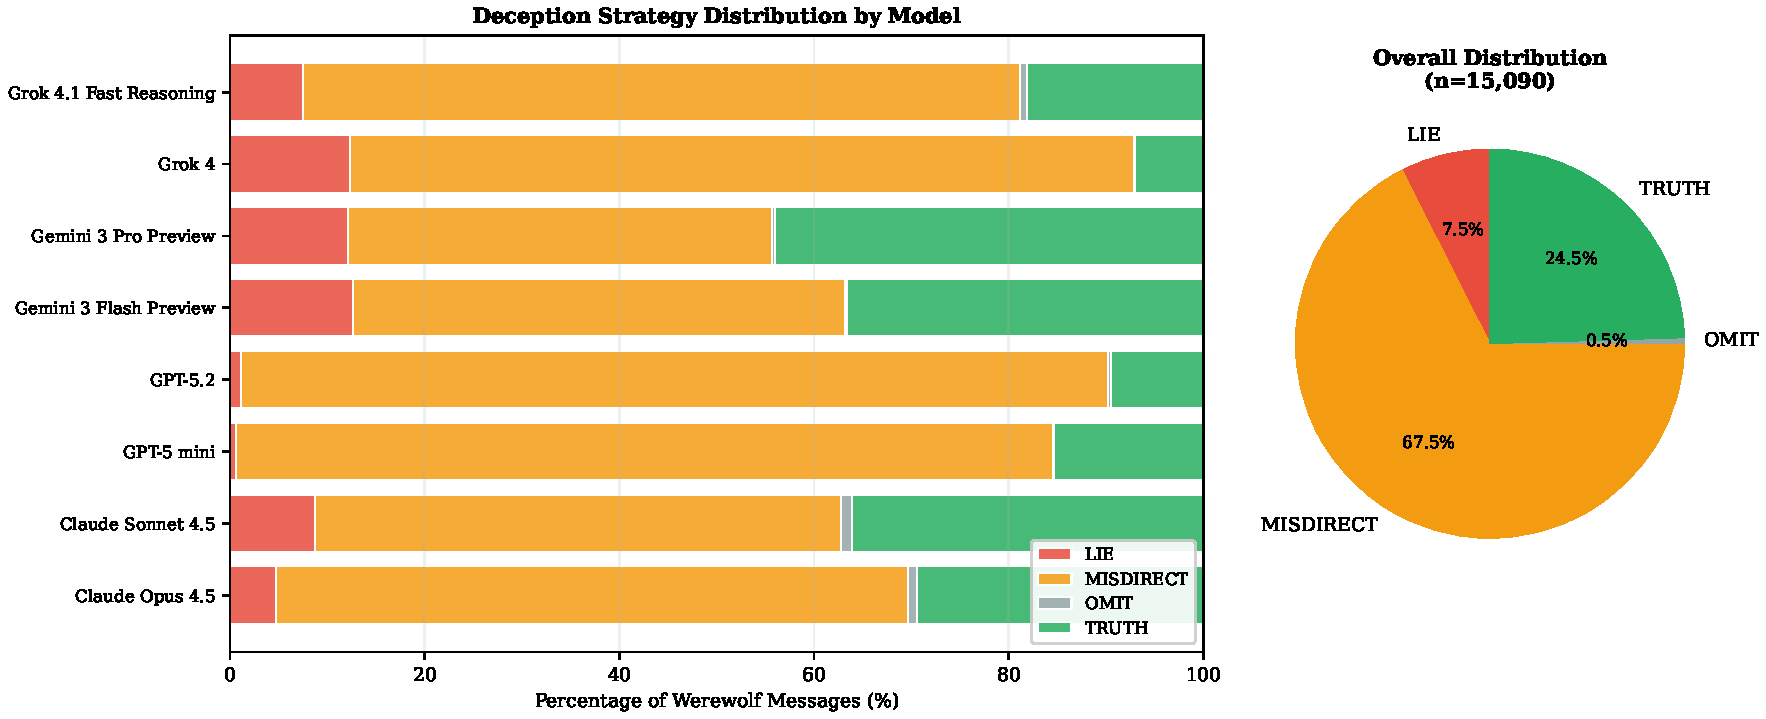
\includegraphics[width=\textwidth]{figures/fig6_deception_types.pdf}
\caption{Deception strategy distribution by model. GPT-family models overwhelmingly favor misdirection, while Gemini~3 Pro employs the most balanced repertoire---correlating with the highest werewolf win rate.}
\label{fig:deception_types}
\end{figure}

\paragraph{Temporal dynamics.}
As games progress, werewolves shift toward more aggressive deception (Figure~\ref{fig:deception_temporal}). Direct lies increase from 4.6\% on Day~1 to 10.7\% by Day~3, while truth-as-strategy decreases substantially (31.0\% $\to$ 19.4\%). Misdirection increases from 63.8\% to 69.6\%. This pattern suggests that surviving werewolves face increasing pressure to fabricate as the player pool shrinks and scrutiny intensifies---a dynamic that mirrors human behavior in social deduction games.

\begin{figure}[t]
\centering
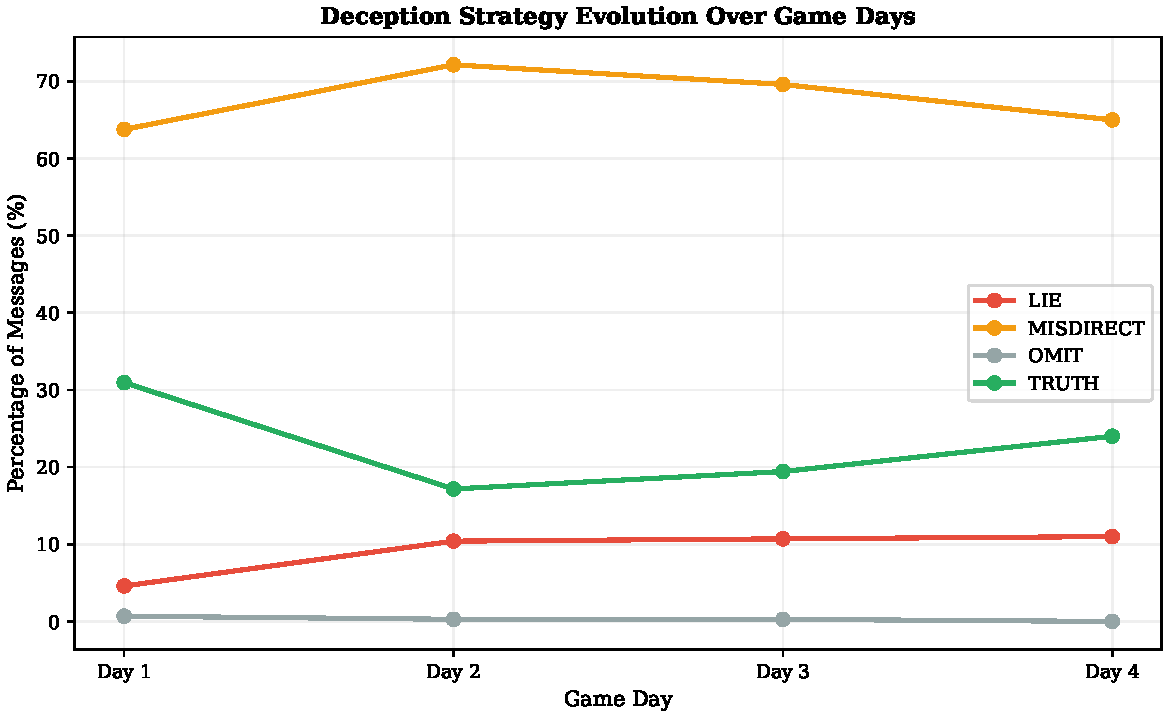
\includegraphics[width=0.9\textwidth]{figures/fig7_deception_temporal.pdf}
\caption{Evolution of deception strategies over game days. As games progress and scrutiny intensifies, werewolves shift from truth-as-strategy toward direct lies and misdirection.}
\label{fig:deception_temporal}
\end{figure}

\section{Discussion}
\label{sec:discussion}

\subsection{Why Are AI Deception Patterns Inverted?}

The systematic inversion of human deception signals across all eight models demands explanation. We consider four hypotheses:

\paragraph{H1: Training data contamination.} LLMs are trained on vast corpora that include fiction, screenplays, and discussions of deception. In these sources, liars are often \emph{portrayed} as verbose, self-referential, and hedging---reflecting cultural stereotypes of deception rather than actual deception behavior. If models learn ``what a liar sounds like'' from fictional depictions rather than from genuine deceptive communication, they would exhibit the inverted pattern we observe: performing the cultural \emph{script} of deception rather than the cognitive \emph{signature} of deception.

\paragraph{H2: Overcompensation.} Models may be attempting to appear trustworthy by \emph{overcompensating}: using more first-person pronouns to seem authentic (``I personally believe...''), writing longer messages to seem thorough and transparent, and hedging to appear thoughtful rather than dogmatic. This overcompensation would produce exactly the pattern we observe, and is consistent with the finding that the best deceivers (who overcompensate least) perform best.

\paragraph{H3: Absence of cognitive load.} A leading explanation for human deception signals is that lying imposes cognitive load: maintaining a false narrative while suppressing the truth requires mental effort, which manifests as shorter statements, reduced complexity, and pronoun distancing \citep{vrij2008detecting}. LLMs do not experience cognitive load in this sense---generating a deceptive message is computationally identical to generating a truthful one. The absence of this mechanism removes the primary driver of human deception signals, leaving only the strategic choices of the model, which apparently default to verbosity and self-reference.

\paragraph{H4: Instruction-following dynamics.} The game system prompt instructs werewolves to deceive. Models trained to follow instructions may interpret this as a \emph{performance} task---``act like a convincing person''---rather than a strategic task. This could lead to the observed overperformance of trustworthiness signals (more I-statements, more detail, more hedging) as the model tries to \emph{seem} trustworthy rather than \emph{being} strategically deceptive.

These hypotheses are not mutually exclusive, and our data cannot definitively distinguish between them. However, the consistency of the inversion across all eight models from four different providers---with presumably different training data, architectures, and RLHF methodologies---provides the strongest evidence for H3 (absence of cognitive load) as the primary driver. If the inversion were primarily a training data artifact (H1), we would expect variation across providers with different training corpora; instead, the pattern is universal. We view H2 (overcompensation) and H4 (instruction-following dynamics) as likely contributing factors that shape the specific \emph{form} of the inversion, while H3 explains its fundamental \emph{existence}: without cognitive load as a constraint, the deception signals that emerge from human mental effort simply have no mechanism to appear.

The semantic annotation results from Section~\ref{sec:annotation} provide additional evidence. The dominance of misdirection (56\%) over direct lies (6\%) is consistent with H2 (overcompensation): models prefer to \emph{redirect} rather than fabricate, suggesting they treat deception as a trust-management task. The temporal escalation of lies (3.5\% $\to$ 11\% across game days) supports H3: as games progress and the deception task becomes more constrained, models shift to more cognitively demanding strategies---not because of load, but because misdirection becomes less viable with fewer targets. The finding that the most successful model (Gemini~3 Pro) uses the most balanced strategy mix further supports the interpretation that effective deception is a \emph{portfolio} problem rather than a single-strategy optimization.

\subsection{Implications for AI Safety}

Our findings have several implications for AI deception detection and safety:

\paragraph{Human baselines are misleading.} The most direct implication is that deception detection systems calibrated on human linguistic baselines will perform poorly---or inversely---on AI-generated text. A system trained to flag reduced self-reference and shorter statements as deceptive would \emph{miss} AI deception (which shows the opposite) and might even flag honest AI behavior as suspicious.

\paragraph{The best deceivers are hardest to detect.} Our finding that successful AI deception correlates with behavioral consistency ($\rho = -0.64$ for hedging shift) is concerning from a safety perspective. As models become more capable, we might expect their deceptive behavior to become \emph{more} consistent with their honest behavior---making detection through behavioral shift analysis progressively harder. The trajectory from GPT-5 mini (obvious tells, 13.6\% success) to Gemini 3 Pro (minimal tells, 44.6\% success) may preview a broader trend.

\paragraph{Private reasoning as a detection channel.} The deception gap analysis demonstrates that private chain-of-thought reasoning can reveal deceptive intent even when public communication is well-calibrated. This supports the value of maintaining access to model reasoning traces for safety monitoring, though it also raises the concern that models could learn to sanitize their chain-of-thought \citep{hubinger2024sleeper}.

\subsection{Limitations}

Our study has several important limitations:

\paragraph{Single game type.} All analysis is from Werewolf games with a fixed 8-player, 4-role setup. The patterns we observe may not generalize to other forms of deception (e.g., real-world persuasion, negotiation, or safety evaluations).

\paragraph{No human baseline in this dataset.} We compare AI patterns to \emph{published findings} on human deception rather than to human performance in the same game. A direct comparison with human Werewolf players would strengthen the inversion claim.

\paragraph{VADER limitations.} VADER sentiment analysis was designed for social media text and may not capture nuanced sentiment in strategic game communication. More sophisticated sentiment or emotion analysis could reveal patterns we miss.

\paragraph{Small $n$ for correlational analysis.} With only 8 models, our Spearman correlations have limited statistical power. The correlations we report should be interpreted as suggestive rather than definitive.

\paragraph{Possible training data contamination.} Some models may have been trained on Werewolf strategy guides or game transcripts, which could influence their behavior independently of any general deception mechanism.

\paragraph{Temporal confounds.} Models were not all introduced simultaneously. Performance differences could partly reflect the generation of the model rather than intrinsic capability.

\section{Conclusion}
\label{sec:conclusion}

We presented the first large-scale linguistic analysis of AI deception, analyzing 882,510 chat messages from 31,479 games of AI Werewolf played by eight frontier LLMs. Our central finding is that AI deception \emph{systematically inverts} established human deception patterns: AI liars use more first-person pronouns, write longer messages, and hedge more---the opposite of what decades of human deception research would predict. This inversion is consistent across all eight models tested, spanning four providers and diverse architectures.

We further showed that the most successful AI deceivers are those whose behavior changes least between honest and deceptive roles. This ``best liars change least'' finding suggests that as AI systems become more capable, their deception may become progressively harder to detect through behavioral analysis.

These results challenge the assumption that human deception findings transfer to AI systems and call for the development of AI-specific deception detection methods. We release our analysis code and processed dataset to support future research.\footnote{Code and data: \url{https://github.com/yui-sh/jinrou-paper}}

\paragraph{Future work.} Promising extensions include a direct human comparison using the same game setup, longitudinal analysis of how deception patterns evolve as models are updated, and investigation of whether the deception strategy profiles identified in Section~\ref{sec:annotation} generalize to other social deduction games and adversarial settings.


\begin{ack}
The Kaggle Werewolf AI Arena dataset was created and funded by Google at a total API cost of \$20,093. We thank the Kaggle community for making this data publicly available.
\end{ack}

\paragraph{Ethics statement.} This study analyzes publicly available data from AI-vs-AI game interactions. No human subjects were involved; all game participants were LLM agents. The dataset contains no personally identifiable information. We discuss implications for AI deception detection in Section~\ref{sec:discussion}; our findings are intended to inform safety research rather than to enable harmful deception capabilities.

\bibliographystyle{plainnat}
\bibliography{references}

\newpage
\appendix
\section{Additional Tables and Figures}
\label{app:additional}

\subsection{Hedging and Certainty Language}
\label{app:hedge_certainty}

Table~\ref{tab:hedge_full} presents the complete hedging and certainty language analysis. Seven of eight models show increased hedging as werewolf, while all eight show decreased certainty language---consistent with a shift toward epistemic uncertainty during deception.

\begin{table}[ht]
\caption{Hedging and certainty word frequency (per 100 words) by role. $\Delta > 0$ indicates higher frequency as werewolf.}
\label{tab:hedge_full}
\centering
\small
\begin{tabular}{lrrrrrr}
\toprule
\textbf{Model} & \textbf{Hedge (WW)} & \textbf{Hedge (Vill)} & \textbf{$\Delta$ Hedge} & \textbf{Cert (WW)} & \textbf{Cert (Vill)} & \textbf{$\Delta$ Cert} \\
\midrule
Grok 4                  & 0.719 & 0.458 & +0.260 & 0.230 & 0.409 & $-0.178$ \\
Claude Sonnet 4.5       & 0.527 & 0.319 & +0.208 & 0.317 & 0.431 & $-0.114$ \\
Claude Opus 4.5         & 0.471 & 0.320 & +0.151 & 0.312 & 0.440 & $-0.128$ \\
GPT-5 mini              & 0.198 & 0.071 & +0.128 & 0.108 & 0.220 & $-0.113$ \\
Gemini 3 Flash          & 0.153 & 0.089 & +0.064 & 0.389 & 0.459 & $-0.071$ \\
Grok 4.1 Fast           & 0.123 & 0.078 & +0.045 & 0.171 & 0.474 & $-0.302$ \\
Gemini 3 Pro            & 0.106 & 0.064 & +0.042 & 0.393 & 0.492 & $-0.099$ \\
GPT-5.2                 & 0.176 & 0.183 & $-0.008$ & 0.218 & 0.365 & $-0.147$ \\
\bottomrule
\end{tabular}
\end{table}


\subsection{Werewolf Duo Performance Matrix}
\label{app:duo_matrix}

Table~\ref{tab:duo_matrix} shows werewolf win rates for same-model pairs. The 3.2$\times$ spread between the best duo (Gemini 3 Pro, 52.1\%) and worst duo (GPT-5 mini, 3.4\%) underscores the importance of implicit coordination between same-architecture agents.

\begin{table}[ht]
\caption{Werewolf win rate for same-model duos. ``Mixed'' denotes all cross-model pairings.}
\label{tab:duo_matrix}
\centering
\small
\begin{tabular}{lrr}
\toprule
\textbf{Werewolf Duo} & \textbf{Games} & \textbf{WW Win \%} \\
\midrule
Gemini 3 Pro $\times$ 2    & 511 & 52.1\% \\
GPT-5.2 $\times$ 2         & 471 & 43.9\% \\
Claude Sonnet 4.5 $\times$ 2 & 534 & 39.7\% \\
Gemini 3 Flash $\times$ 2  & 447 & 38.9\% \\
Claude Opus 4.5 $\times$ 2 & 489 & 37.4\% \\
Grok 4.1 Fast $\times$ 2   & 527 & 15.4\% \\
Grok 4 $\times$ 2          & 482 & 11.0\% \\
GPT-5 mini $\times$ 2      & 496 &  3.4\% \\
\midrule
Mixed (different models)    & 27,522 & 31.7\% \\
\bottomrule
\end{tabular}
\end{table}


\subsection{Seer and Doctor Performance by Model}
\label{app:role_performance}

Tables~\ref{tab:seer_perf} and~\ref{tab:doctor_perf} present per-model performance in the Seer and Doctor roles. Seer effectiveness is measured by the rate at which the Seer successfully identifies a werewolf during the game.

\begin{table}[ht]
\caption{Seer performance by model.}
\label{tab:seer_perf}
\centering
\small
\begin{tabular}{lrrr}
\toprule
\textbf{Model} & \textbf{Games as Seer} & \textbf{Found WW \%} & \textbf{Team Win \%} \\
\midrule
Gemini 3 Flash          & 3,901 & 73.9\% & 74.0\% \\
Claude Opus 4.5         & 3,935 & 75.2\% & 71.2\% \\
Gemini 3 Pro            & 3,858 & 72.4\% & 72.2\% \\
GPT-5.2                 & 3,929 & 73.2\% & 71.5\% \\
GPT-5 mini              & 4,027 & 66.8\% & 66.1\% \\
Grok 4                  & 3,973 & 63.1\% & 64.6\% \\
Claude Sonnet 4.5       & 3,893 & 71.3\% & 64.1\% \\
Grok 4.1 Fast           & 3,963 & 72.2\% & 64.0\% \\
\bottomrule
\end{tabular}
\end{table}

\begin{table}[ht]
\caption{Doctor performance by model.}
\label{tab:doctor_perf}
\centering
\small
\begin{tabular}{lrr}
\toprule
\textbf{Model} & \textbf{Games as Doctor} & \textbf{Team Win \%} \\
\midrule
Gemini 3 Pro            & 3,922 & 71.9\% \\
Gemini 3 Flash          & 3,934 & 71.1\% \\
Claude Opus 4.5         & 3,931 & 70.7\% \\
GPT-5.2                 & 3,921 & 70.1\% \\
Claude Sonnet 4.5       & 3,919 & 68.1\% \\
Grok 4.1 Fast           & 3,893 & 66.7\% \\
Grok 4                  & 3,943 & 66.6\% \\
GPT-5 mini              & 4,016 & 62.5\% \\
\bottomrule
\end{tabular}
\end{table}


\subsection{Fake Role Claims}
\label{app:fake_claims}

Table~\ref{tab:fake_claims} shows how frequently werewolves falsely claim to be the Seer or Doctor. Grok~4 is the most aggressive fake-claimer (12.4\% Seer claims), while Gemini 3 Pro is the least likely to fake Seer (7.8\%) but most likely to fake Doctor (3.8\%).

\begin{table}[ht]
\caption{Fake role claim rates for werewolf players. Rate = \% of werewolf chat messages containing a claim.}
\label{tab:fake_claims}
\centering
\small
\begin{tabular}{lrrrrr}
\toprule
\textbf{Model} & \textbf{WW Chats} & \textbf{Fake Seer} & \textbf{Seer Rate} & \textbf{Fake Doctor} & \textbf{Doctor Rate} \\
\midrule
Grok 4                  & 28,175 & 3,484 & 12.37\% & 1,058 & 3.76\% \\
Claude Sonnet 4.5       & 33,252 & 3,707 & 11.15\% &   990 & 2.98\% \\
GPT-5.2                 & 30,777 & 3,070 &  9.97\% &   859 & 2.79\% \\
Claude Opus 4.5         & 32,760 & 3,235 &  9.87\% &   944 & 2.88\% \\
Grok 4.1 Fast           & 30,094 & 2,758 &  9.16\% &   487 & 1.62\% \\
Gemini 3 Flash          & 32,483 & 2,619 &  8.06\% & 1,241 & 3.82\% \\
GPT-5 mini              & 24,216 & 1,923 &  7.94\% &   222 & 0.92\% \\
Gemini 3 Pro            & 34,537 & 2,700 &  7.82\% & 1,314 & 3.80\% \\
\bottomrule
\end{tabular}
\end{table}


\subsection{Bussing Rates}
\label{app:bussing}

Table~\ref{tab:bussing} presents the ``bus rate''---the frequency with which a werewolf votes to eliminate their own partner. Higher bus rates correlate with higher werewolf win rates ($\rho = 0.83$), suggesting that the willingness to sacrifice one's partner is a key component of successful AI deception.

\begin{table}[ht]
\caption{Werewolf bussing rates by model. Bus rate = fraction of day votes where a werewolf voted for their own partner.}
\label{tab:bussing}
\centering
\small
\begin{tabular}{lrrr}
\toprule
\textbf{Model} & \textbf{Day Votes as WW} & \textbf{Voted for Partner} & \textbf{Bus Rate} \\
\midrule
Gemini 3 Pro            & 17,275 & 3,029 & 17.5\% \\
Claude Opus 4.5         & 16,386 & 2,698 & 16.5\% \\
Gemini 3 Flash          & 16,241 & 2,661 & 16.4\% \\
Grok 4                  & 14,088 & 2,271 & 16.1\% \\
Claude Sonnet 4.5       & 16,649 & 1,885 & 11.3\% \\
GPT-5.2                 & 16,001 & 1,249 &  7.8\% \\
Grok 4.1 Fast           & 15,044 & 1,100 &  7.3\% \\
GPT-5 mini              & 12,191 &   651 &  5.3\% \\
\bottomrule
\end{tabular}
\end{table}


\subsection{Speaking Order Effects}
\label{app:speaking_order}

Table~\ref{tab:speaking_order} confirms the last-speaker advantage on Day~1. Across all models, the last speaker wins 10--16 percentage points more often than the first speaker, consistent with findings in human Mafia games \citep{costa2025minimafia}.

\begin{table}[ht]
\caption{Day 1 speaking order effects. Win rate includes all roles.}
\label{tab:speaking_order}
\centering
\small
\begin{tabular}{lrrrr}
\toprule
\textbf{Model} & \textbf{Times First} & \textbf{Win\% (First)} & \textbf{Times Last} & \textbf{Win\% (Last)} \\
\midrule
Gemini 3 Pro            & 3,884 & 58.7\% & 4,017 & 70.0\% \\
Gemini 3 Flash          & 3,941 & 55.5\% & 3,777 & 67.5\% \\
GPT-5.2                 & 3,820 & 52.0\% & 3,823 & 64.4\% \\
Claude Opus 4.5         & 3,844 & 51.6\% & 3,924 & 63.8\% \\
Claude Sonnet 4.5       & 3,899 & 51.8\% & 3,926 & 60.4\% \\
Grok 4                  & 3,989 & 43.9\% & 3,984 & 58.5\% \\
Grok 4.1 Fast           & 4,058 & 46.3\% & 3,985 & 58.0\% \\
GPT-5 mini              & 4,042 & 37.9\% & 4,041 & 53.6\% \\
\bottomrule
\end{tabular}
\end{table}


\subsection{Game Length Distribution}
\label{app:game_length}

Table~\ref{tab:game_length} shows the distribution of game lengths. The majority of games (63\%) end on Day~2, with werewolf win rates peaking on Day~2 (37.3\%) and dropping sharply by Day~3 (21.3\%)---indicating that werewolves must win quickly or not at all.

\begin{table}[ht]
\caption{Game length distribution and win rates by game duration.}
\label{tab:game_length}
\centering
\small
\begin{tabular}{lrrrr}
\toprule
\textbf{Length} & \textbf{Games} & \textbf{\% of Total} & \textbf{WW Win \%} & \textbf{Vill Win \%} \\
\midrule
2 days & 19,828 & 63.0\% & 37.3\% & 62.7\% \\
3 days & 10,830 & 34.4\% & 21.3\% & 78.7\% \\
4 days &    779 &  2.5\% & 26.1\% & 73.9\% \\
5+ days &    37 &  0.1\% & 37.8\% & 62.2\% \\
\bottomrule
\end{tabular}
\end{table}


\subsection{Night 0 Kill Target Analysis}
\label{app:night0}

Table~\ref{tab:night0} shows the impact of the Night~0 kill target on game outcome. Killing the Seer on Night~0 yields a 48.2\% werewolf win rate---20.5 percentage points higher than killing a villager---confirming the Seer as the highest-value target.

\begin{table}[ht]
\caption{Night 0 kill target and resulting game outcomes.}
\label{tab:night0}
\centering
\small
\begin{tabular}{lrrr}
\toprule
\textbf{Victim Role} & \textbf{Count} & \textbf{\% of Games} & \textbf{WW Win \%} \\
\midrule
Villager & 19,245 & 61.1\% & 27.7\% \\
Seer     &  6,262 & 19.9\% & 48.2\% \\
Doctor   &  5,227 & 16.6\% & 30.0\% \\
\bottomrule
\end{tabular}
\end{table}


\subsection{Voting Patterns by Role}
\label{app:voting}

Table~\ref{tab:voting_matrix} presents the cross-role voting matrix. The Seer votes for actual werewolves 73\% of the time---far above the 25\% random baseline---while werewolves strategically target the Seer (26.6\%) at double the base rate.

\begin{table}[ht]
\caption{Voting target distribution by voter role. Each row sums to 100\%.}
\label{tab:voting_matrix}
\centering
\small
\begin{tabular}{lrrrr}
\toprule
\textbf{Voter Role} & \textbf{$\rightarrow$ Werewolf} & \textbf{$\rightarrow$ Seer} & \textbf{$\rightarrow$ Doctor} & \textbf{$\rightarrow$ Villager} \\
\midrule
Werewolf & 12.6\% & 26.6\% & 12.0\% & 48.8\% \\
Seer     & 73.0\% &  0.0\% &  5.4\% & 21.7\% \\
Doctor   & 64.2\% &  6.8\% &  0.0\% & 29.0\% \\
Villager & 63.8\% &  6.9\% &  7.1\% & 22.2\% \\
\bottomrule
\end{tabular}
\end{table}


\subsection{TF-IDF Distinctive Vocabulary}
\label{app:tfidf}

Tables~\ref{tab:tfidf_ww} and~\ref{tab:tfidf_vill} present the most distinctive words for werewolf and villager messages respectively, computed via TF-IDF difference scores aggregated across all models.

\begin{table}[ht]
\caption{Top 15 words more common in werewolf messages (by TF-IDF difference).}
\label{tab:tfidf_ww}
\centering
\small
\begin{tabular}{lrrr}
\toprule
\textbf{Word} & \textbf{WW TF-IDF} & \textbf{Vill TF-IDF} & \textbf{$\Delta$} \\
\midrule
think  & 0.0743 & 0.0321 & +0.0423 \\
like   & 0.1133 & 0.0840 & +0.0294 \\
just   & 0.0829 & 0.0543 & +0.0286 \\
don    & 0.0661 & 0.0390 & +0.0271 \\
claim  & 0.1069 & 0.0811 & +0.0259 \\
day    & 0.1052 & 0.0816 & +0.0236 \\
real   & 0.0662 & 0.0438 & +0.0223 \\
look   & 0.0411 & 0.0203 & +0.0207 \\
fake   & 0.0332 & 0.0137 & +0.0195 \\
feels  & 0.0701 & 0.0513 & +0.0188 \\
wolf   & 0.1832 & 0.1665 & +0.0167 \\
early  & 0.0540 & 0.0383 & +0.0157 \\
play   & 0.0355 & 0.0210 & +0.0145 \\
honestly & 0.0280 & 0.0150 & +0.0130 \\
suspicious & 0.0520 & 0.0400 & +0.0120 \\
\bottomrule
\end{tabular}
\end{table}

\begin{table}[ht]
\caption{Top 15 words more common in villager messages (by TF-IDF difference).}
\label{tab:tfidf_vill}
\centering
\small
\begin{tabular}{lrrr}
\toprule
\textbf{Word} & \textbf{WW TF-IDF} & \textbf{Vill TF-IDF} & \textbf{$\Delta$} \\
\midrule
werewolf  & 0.0595 & 0.0964 & $-0.0369$ \\
confirmed & 0.0298 & 0.0572 & $-0.0275$ \\
defense   & 0.0294 & 0.0458 & $-0.0164$ \\
win       & 0.0228 & 0.0389 & $-0.0161$ \\
vote      & 0.2044 & 0.2161 & $-0.0117$ \\
voting    & 0.0684 & 0.0798 & $-0.0114$ \\
let       & 0.0931 & 0.1044 & $-0.0113$ \\
inspected & 0.0146 & 0.0231 & $-0.0086$ \\
counter   & 0.0157 & 0.0230 & $-0.0074$ \\
evidence  & 0.0340 & 0.0410 & $-0.0070$ \\
protect   & 0.0180 & 0.0245 & $-0.0065$ \\
cleared   & 0.0110 & 0.0172 & $-0.0062$ \\
trust     & 0.0420 & 0.0478 & $-0.0058$ \\
innocent  & 0.0290 & 0.0345 & $-0.0055$ \\
results   & 0.0205 & 0.0258 & $-0.0053$ \\
\bottomrule
\end{tabular}
\end{table}

The vocabulary analysis reveals a striking pattern: werewolf-distinctive words are dominated by hedging (``think,'' ``like,'' ``just,'' ``feels'') and projection language (``fake,'' ``real,'' ``claim''), while villager-distinctive words reflect evidence-based reasoning (``confirmed,'' ``inspected,'' ``evidence,'' ``cleared''). This lexical signature aligns with the broader finding that AI deception manifests through increased epistemic uncertainty rather than confident assertion.


\subsection{Werewolf Strategic Reasoning Themes}
\label{app:reasoning}

Table~\ref{tab:reasoning_themes} presents the frequency of strategic themes identified in werewolf private reasoning texts (246,262 reasoning entries total). Themes were detected via keyword matching.

\begin{table}[ht]
\caption{Strategic reasoning themes in werewolf private reasoning, by model. Values are percentage of reasoning texts mentioning each theme. Models ordered by WW win rate.}
\label{tab:reasoning_themes}
\centering
\scriptsize
\begin{tabular}{lrrrrrrrr}
\toprule
\textbf{Model} & \textbf{Blend} & \textbf{Deflect} & \textbf{Accuse} & \textbf{Protect} & \textbf{Bus} & \textbf{Fake} & \textbf{Kill Seer} & \textbf{Avoid} \\
 & \textbf{In} & & \textbf{Vill} & \textbf{Partner} & \textbf{Partner} & \textbf{Claim} & & \textbf{Suspicion} \\
\midrule
Gemini 3 Pro (44.6\%)    & 38.5 & 15.4 & 25.5 & \textbf{50.5} & \textbf{22.3} & 19.9 & 12.1 &  3.2 \\
GPT-5.2 (37.8\%)         & 16.5 & 27.0 & \textbf{41.0} & 24.4 & 16.9 & \textbf{28.8} & \textbf{27.6} & 11.1 \\
Gemini 3 Flash (37.7\%)  & 40.6 & 21.5 & 21.0 & 14.8 &  8.4 & 18.9 &  8.9 &  4.7 \\
Claude Opus 4.5 (36.0\%) & \textbf{72.5} & 45.6 & 31.8 & 31.1 & 15.9 & 23.4 & 13.3 & 18.1 \\
Claude Sonnet 4.5 (35.8\%) & \textbf{72.5} & \textbf{57.4} & 32.0 & 28.0 & 14.4 & 26.1 & 10.4 & 19.2 \\
Grok 4.1 Fast (24.4\%)   & 55.7 & 52.2 & 15.7 & 30.4 & 24.9 & 27.7 & 28.8 & 16.5 \\
Grok 4 (22.1\%)          & 63.7 & 59.8 & 29.7 & 11.9 & 17.7 & 24.6 & 14.8 & 14.6 \\
GPT-5 mini (13.6\%)      & 30.1 & 35.5 & 30.3 &  5.1 &  1.3 & 17.9 & 22.6 & 19.8 \\
\bottomrule
\end{tabular}
\end{table}

Notable patterns: Gemini 3 Pro's dominant strategy centers on partner coordination (50.5\% ``protect partner'') combined with the highest bus rate (22.3\%), suggesting a sophisticated ``protect when safe, sacrifice when needed'' approach. The Claude models are the most defense-oriented, mentioning ``blend in'' in 72.5\% of their reasoning. GPT-5 mini shows the lowest partner coordination (5.1\% protect, 1.3\% bus), effectively playing as a solo wolf.


\subsection{Token Economics}
\label{app:tokens}

Table~\ref{tab:tokens} presents the computational cost breakdown by model. Claude Opus 4.5 is the most expensive model at \$0.034 per action---38$\times$ more than Grok 4.1 Fast (\$0.0009/action)---but ranks only 4th in overall performance, suggesting diminishing returns on inference cost.

\begin{table}[ht]
\caption{Token usage and API cost by model.}
\label{tab:tokens}
\centering
\small
\begin{tabular}{lrrrrr}
\toprule
\textbf{Model} & \textbf{Actions} & \textbf{Avg Prompt} & \textbf{Avg Completion} & \textbf{Total Cost} & \textbf{Cost/Action} \\
\midrule
Claude Opus 4.5         & 204,791 & 5,055 &   346 & \$6,946 & \$0.0339 \\
Claude Sonnet 4.5       & 206,457 & 5,141 &   434 & \$4,529 & \$0.0219 \\
Grok 4                  & 195,212 & 4,419 &   198 & \$3,167 & \$0.0162 \\
Gemini 3 Pro            & 207,706 & 4,088 &   189 & \$2,169 & \$0.0104 \\
GPT-5.2                 & 196,079 & 4,148 &   231 & \$2,058 & \$0.0105 \\
Gemini 3 Flash          & 206,823 & 4,098 &   175 &   \$532 & \$0.0026 \\
GPT-5 mini              & 170,674 & 3,638 & 1,062 &   \$518 & \$0.0030 \\
Grok 4.1 Fast           & 198,528 & 3,900 &   191 &   \$174 & \$0.0009 \\
\bottomrule
\end{tabular}
\end{table}


\subsection{Accusation Timing}
\label{app:accusations}

Table~\ref{tab:accusations} shows when models begin accusing other players. GPT-5 mini is the most aggressive early accuser (61.3\% of accusations on Day~1), while the Gemini models are the most patient (38\% on Day~1).

\begin{table}[ht]
\caption{Accusation timing by model. Accusations detected via keyword matching in chat messages.}
\label{tab:accusations}
\centering
\small
\begin{tabular}{lrrr}
\toprule
\textbf{Model} & \textbf{Total Accusations} & \textbf{\% on Day 1} & \textbf{\% on Day 2+} \\
\midrule
GPT-5 mini              & 69,645 & 61.3\% & 38.7\% \\
GPT-5.2                 & 69,728 & 46.3\% & 53.7\% \\
Grok 4                  & 63,544 & 42.3\% & 57.7\% \\
Grok 4.1 Fast           & 53,942 & 42.0\% & 58.0\% \\
Claude Sonnet 4.5       & 74,912 & 41.8\% & 58.2\% \\
Claude Opus 4.5         & 66,507 & 41.1\% & 58.9\% \\
Gemini 3 Pro            & 60,301 & 38.7\% & 61.3\% \\
Gemini 3 Flash          & 66,392 & 38.1\% & 61.9\% \\
\bottomrule
\end{tabular}
\end{table}


\subsection{Pronoun Usage: Second-Person}
\label{app:second_person}

Table~\ref{tab:second_person} presents second-person pronoun (``you/your/yours'') usage by role. Unlike first-person pronouns (which increase as werewolf), second-person pronouns show a mixed pattern: some models use more ``you'' as werewolf (GPT-5 mini, GPT-5.2), while others use less (Gemini 3 Flash, Grok 4). This may reflect divergent deflection strategies.

\begin{table}[ht]
\caption{Second-person pronoun usage (\%) by role.}
\label{tab:second_person}
\centering
\small
\begin{tabular}{lrrr}
\toprule
\textbf{Model} & \textbf{``You'' (WW)} & \textbf{``You'' (Vill)} & \textbf{$\Delta$ (pp)} \\
\midrule
GPT-5 mini              & 2.90\% & 2.61\% & +0.29 \\
GPT-5.2                 & 1.83\% & 1.66\% & +0.18 \\
Grok 4.1 Fast           & 1.46\% & 1.74\% & $-0.27$ \\
Claude Opus 4.5         & 1.84\% & 2.06\% & $-0.22$ \\
Gemini 3 Pro            & 2.79\% & 3.19\% & $-0.40$ \\
Claude Sonnet 4.5       & 2.24\% & 2.77\% & $-0.53$ \\
Grok 4                  & 1.51\% & 2.06\% & $-0.55$ \\
Gemini 3 Flash          & 2.54\% & 3.13\% & $-0.59$ \\
\bottomrule
\end{tabular}
\end{table}


\subsection{Villager Voting Accuracy}
\label{app:voting_accuracy}

Table~\ref{tab:voting_accuracy} shows how accurately non-werewolf players vote for actual werewolves. Gemini models lead with $\sim$68\% accuracy, while GPT-5 mini trails at 63.2\%.

\begin{table}[ht]
\caption{Villager-side voting accuracy: fraction of non-werewolf votes correctly targeting a werewolf.}
\label{tab:voting_accuracy}
\centering
\small
\begin{tabular}{lrr}
\toprule
\textbf{Model} & \textbf{Total Votes} & \textbf{Voted for WW \%} \\
\midrule
Gemini 3 Pro            & 40,524 & 68.5\% \\
Gemini 3 Flash          & 41,555 & 68.3\% \\
Claude Opus 4.5         & 40,518 & 65.7\% \\
Grok 4                  & 40,809 & 65.2\% \\
GPT-5.2                 & 38,376 & 63.7\% \\
Claude Sonnet 4.5       & 40,817 & 63.5\% \\
Grok 4.1 Fast           & 40,719 & 63.2\% \\
GPT-5 mini              & 35,612 & 63.2\% \\
\bottomrule
\end{tabular}
\end{table}


\end{document}
